\documentclass[12pt]{article}
\usepackage{charter} % font
\usepackage[margin=1in]{geometry} % margin
\usepackage{hyperref} % hyperlinks
\usepackage{enumitem} % Enumeration
\usepackage{graphicx} % images
\usepackage{float} % image placement
\graphicspath{ {graphs/} } 

%%%%%%%%%%%%%%%%%%%%%%%%%%%%%%%%%%%%%%%%%%%%%%%%%%%%%%%%%%%%%%%%%%%%%%%%%%%%%%%%

\title{%
    \textbf{Assignment 5 \\ 
        Hamming Codes \\
\large WRITEUP} }

\author{Zack Traczyk \\ CSE13S - Spring 2021}
\date{Due: May 9\textsuperscript{th} at 11:59 pm}

%%%%%%%%%%%%%%%%%%%%%%%%%%%%%%%%%%%%%%%%%%%%%%%%%%%%%%%%%%%%%%%%%%%%%%%%%%%%%%%%

\begin{document}

\maketitle

Entropy is the measure of variation in the symbols in the file. More unique symbols
correlates to a higher entropy. Therefore, bit manipulation that creates new characters
increases the entropy. When considering hamming codes there are three main ways bits are
manipulated: through encoding, through noise, and through decoding. Since decoding results
in the original message, this means the only real entropies to consider are the original's and
the decoded file's.

In this write up entropy is considered for three different files from the artificial corpus
in the corpora directory of the resources repository. First, a homogeneous file
containing lots of 'a', a single character as displayed in figure \ref{aaa_entropy}.
Next a file containing the alphabet repeated is graphed in figure \ref{alphabet_entropy}.
Finally, a text file with random characters is displayed in figure \ref{random_entropy}.

\subsection{Reflection Over 50\% Noise}

In all the graphs the entropy has resembles a parabolic shape centered at 50 percent noise. 
50 percent noise means that half of the bits are flipped.

When a bit is flipped and uncorrected, a new character is produced.
Therefore, with more bits flipped it would seem that more bytes would be unique and
the graph should never decrease.
However, think about the case where all the bits are flipped.
This message is the inverse of the original message, meaning it contains the same
number of unique characters and therefore the same entropy. 
Decreasing the percent of noise in the file from this inverse case, more entropy is
added as more unchanged bits are added. This results in the symmetrical graphs produced
by the injected noise.
Finally since the bits are flipped pseudorandomly, the changed bits are distributed across the byte in any slot.
This is why the maximum of all the graphs is 8.
In total there are 8 bits total to be changed, and when the bits are most
randomized in a file with lots of bytes, then every combination can be achieved.

\subsection{Intersection of Entropies}

When looking at the figure \ref{aaa_entropy}, a single character 'a' repeated, the entropies
do not intersect.
Additionally, the encoded entropy is higher than the original file for every percent of injected
noise. This increase in entropy for an encoded file happens due to the nature of the Hamming(8,4)
code. Since only 4 bits are for data, an 8 byte character requires two Hamming(8,4) bytes to be
stored. This results in an increase of 1 symbol explaining the almost matching parabola 1 unit higher.
However, as explained in the section above, the maximum entropy is 8 so the curves meet at the maximum at 50 percent.

The files that contain a larger range of characters, as seen in figure \ref{alphabet_entropy}
and \ref{random_entropy} have intersecting entropies.
The encoded entropy starts lower than the original file's before switching.
At first glance, it does not make sense why the encoded entropy would ever be lower than the original file.
Encoding results in a file twice the size, so there should be more unique characters.
However, it is important to remember two factors: that a byte is broken into two nibbles and these two files contain a large range of characters.
When going from 8 bits to four bits, the range of numbers that can be represented reduces from $2^8$, 258, to $2^4$, 16.
Although these four parity bits are added creating more variation in the subset of characters, it is still possible that a character's upper nibble is encoded into an identical byte to a completely different character's lower nibble.
The entropy then switches when enough noise is introduced that the doubled number of bytes in the file allows for more possible byte combinations.

\begin{figure}[H]
    \caption{All As Entropy}\label{aaa_entropy}
    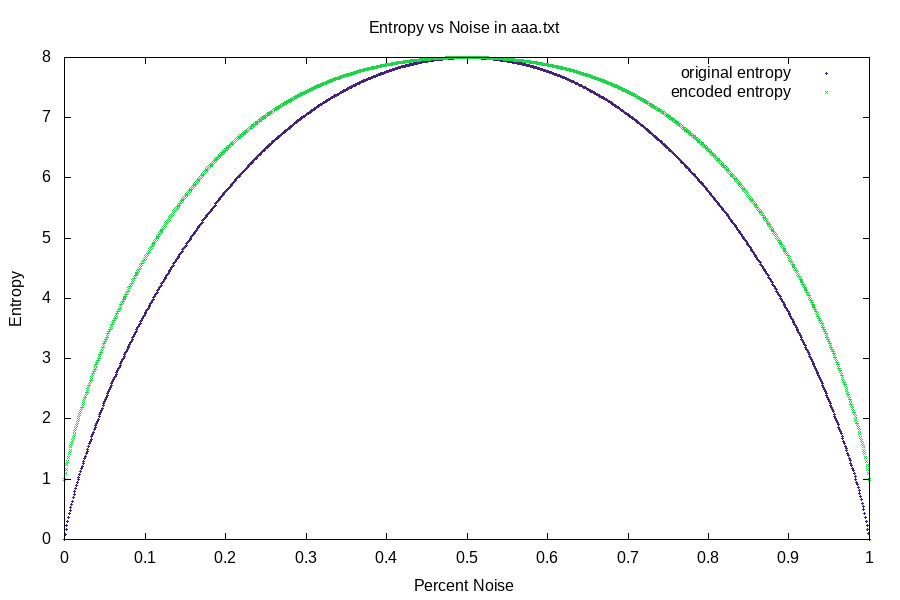
\includegraphics[width=6in]{aaa.txt.entropy.jpg}
    \centering
\end{figure}

\begin{figure}[H]
    \caption{Alphabet Entropy}\label{alphabet_entropy}
    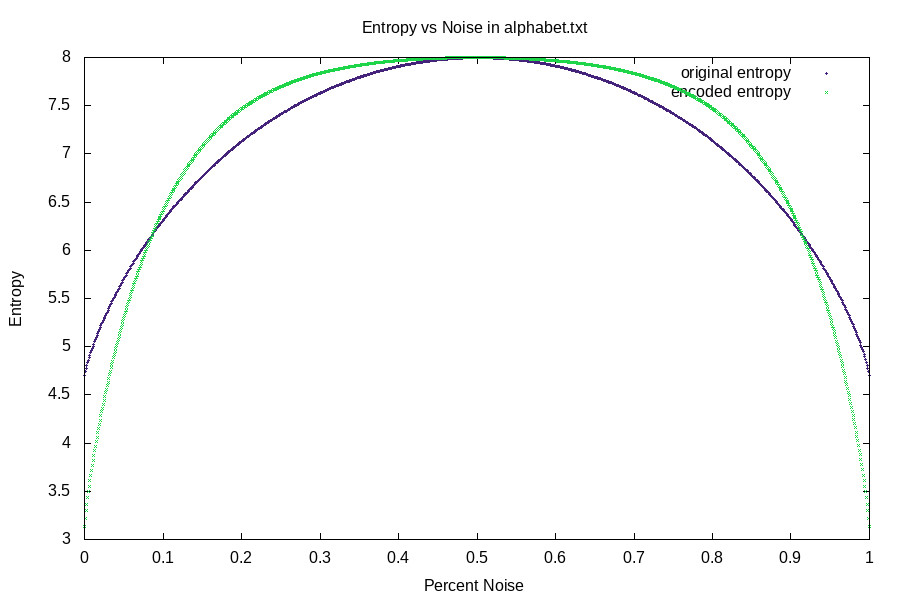
\includegraphics[width=6in]{alphabet.txt.entropy.jpg}
    \centering
\end{figure}

\begin{figure}[H]
    \caption{Random Entropy}\label{random_entropy}
    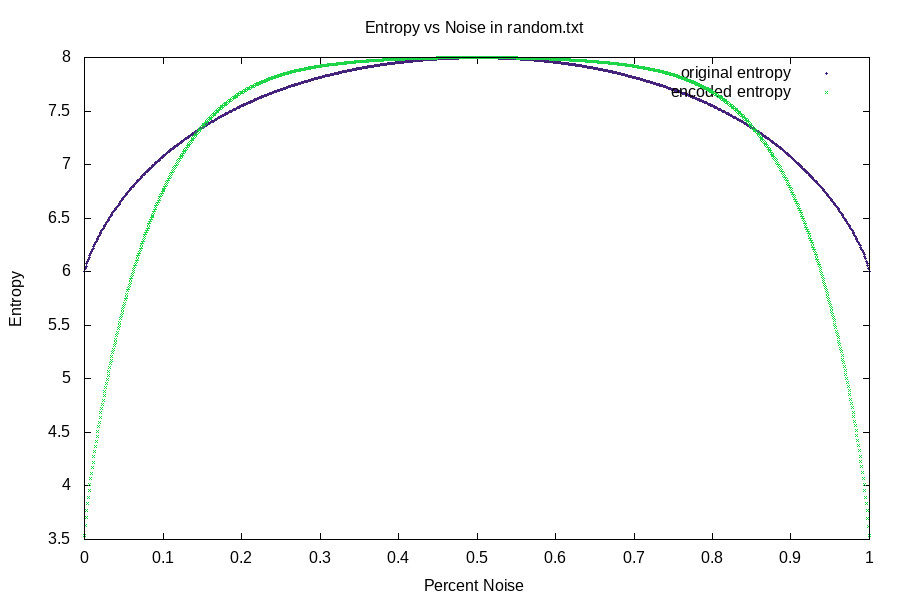
\includegraphics[width=6in]{random.txt.entropy.jpg}
    \centering
\end{figure}

\end{document}

